% ==STYLE-BEGIN==
\documentclass[UTF8,11pt]{ctexart}
\usepackage{amsmath,amssymb,amsthm}
\usepackage[a4paper,margin=2.4cm,top=2.3cm,bottom=2.3cm]{geometry}
\usepackage{fancyhdr}
\usepackage{enumitem}
\usepackage{hyperref}
\hypersetup{hidelinks}

% ---- 版式 ----
\linespread{1.15}
\setlength{\parskip}{0.35em}
\setlength{\parindent}{1.6em}
\setlist{nosep,leftmargin=2em}

% ---- 页眉 ----
\pagestyle{fancy}
\fancyhf{}
\fancyhead[L]{\small\coursename}
\fancyhead[R]{\small\thepage}
\renewcommand{\headrulewidth}{0.4pt}

% ---- 定理环境：中文用正体，标题加粗，按小节共用一条流水号 ----
\newtheoremstyle{cnthm}{0.7em}{0.7em}{\normalfont}{}{\bfseries}{}{0.5em}{}
\theoremstyle{cnthm}
\newtheorem{thm}{定理}[section]
\newtheorem{lem}[thm]{引理}
\newtheorem{prop}[thm]{命题}
\newtheorem{cor}[thm]{推论}
\newtheorem{defn}[thm]{定义}
\newtheorem{rem}[thm]{注}
\newtheorem{exa}[thm]{例}
\newtheorem{conj}[thm]{猜想}
\renewcommand{\proofname}{\bfseries 证明}
\providecommand{\coursename}{}
% ==STYLE-END==
\renewcommand{\coursename}{解析几何\,·\,1010}
\title{几何与代数 1010}
\usepackage{graphicx}
\graphicspath{{../pic/}{pic/}} % 本地在 tex/ 下编译用 ../pic；Overleaf 平铺结构用 pic
\xeCJKDeclareCharClass{CJK}{"2460 -> "2473} % 让 ①②③ 等圈号使用中文字体
\date{}
\begin{document}
\maketitle

\section{\ 旋转面}

\textbf{定义}：平面曲线绕同一平面的直线旋转一周得到的图形。

该曲线称为\textbf{子午线}，直线称为\textbf{轴线}。

\begin{center}
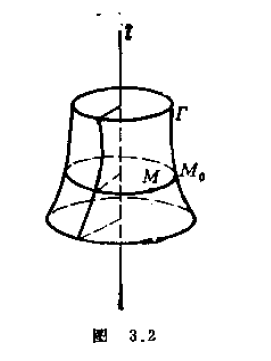
\includegraphics[width=0.36\linewidth]{ga-1010/ga-1.png}
\end{center}

子午线 $P$：
\[
\begin{cases}
f(y,z)=0, \\
x=0 .
\end{cases}
\]

设旋转面为 $S$，方程为 $F(x,y,z)=0$。
$\forall$ 点 $P(x_0,y_0,z_0)\in S$，过点 $P$ 作一平面 $\pi$ 与
$z$ 轴垂直，该平面方程为
\[
z=z_0 .
\]

$\pi$ 与子午线 $P$ 交于点 $P'(0,y_1,z_0)$。又 $P$ 与 $P'$ 到
$z$ 轴距离相同，因此
\[
x_0^2+y_0^2=y_1^2 \Longrightarrow y_1=\pm\sqrt{x_0^2+y_0^2}.
\]

而 $P'\in P$，于是
\[
f\left(\pm\sqrt{x_0^2+y_0^2},\ z_0\right)=0 .
\]

即 $S$ 的方程为
\[
f\left(\pm\sqrt{x^2+y^2},\ z\right)=0 .
\]

\subsubsection*{例 1}

\[
P:\begin{cases}\dfrac{y^2}{a^2}-\dfrac{z^2}{b^2}=1,\\[8pt] x=0 .\end{cases}
\]

\begin{enumerate}
\item $P$ 绕 $z$ 轴旋转，得到旋转面方程为
\[
\frac{x^2+y^2}{a^2}-\frac{z^2}{b^2}=1,
\]
即单叶旋转双曲面。

\begin{center}
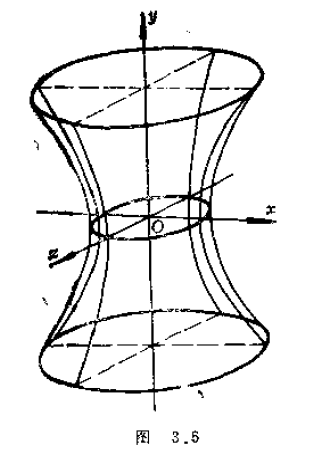
\includegraphics[width=0.36\linewidth]{ga-1010/ga-3.png}
\end{center}

\item $P$ 绕 $y$ 轴旋转一周，得到旋转面方程为
\[
\frac{y^2}{a^2}-\frac{x^2+z^2}{b^2}=1,
\]
即双叶旋转双曲面。

\begin{center}
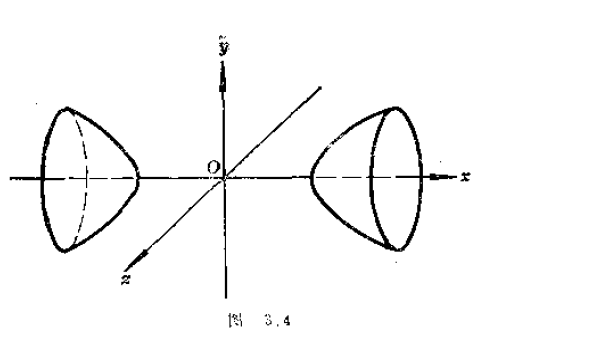
\includegraphics[width=0.36\linewidth]{ga-1010/ga-2.png}
\end{center}
\end{enumerate}

\subsubsection*{例 2：异面直线 $l_1$、$l_2$}

$z$ 轴为 $l_1$，$x$ 轴为公垂线。$l_2$ 与 $x$ 轴交于点 $P(a,0,0)$。
$l_2$ 的方向为 $\vec v=(0,1,c)$，即
\[
l_2:\begin{cases}x=a+0t, \\ y=0+1t, \\ z=0+ct .\end{cases}
\]

设旋转后的图形为 $S$，$\forall$ 点 $Q(x,y,z)$，过点 $Q$ 作平面
$\pi$，它与 $l_2$ 交于点
\[
Q'\left(a,\ \frac{z}{c},\ z\right).
\]

又 $Q$ 与 $Q'$ 到 $z$ 轴距离相等，故
\[
x^2+y^2=a^2+\frac{z^2}{c^2}
\quad\Longleftrightarrow\quad
\frac{x^2+y^2}{a^2}-\frac{z^2}{a^2c^2}=1 .
\]

\subsubsection*{例 3：Möbius 带}

\[
\begin{cases}
x=\left(R-r\sin\dfrac{\theta}{2}\right)\cos\theta,\\[8pt]
y=\left(R-r\sin\dfrac{\theta}{2}\right)\sin\theta,\\[8pt]
z=r\cos\dfrac{\theta}{2},
\end{cases}
\qquad
0\leq\theta\leq2\pi,\qquad -1\leq r\leq1 .
\]

\subsubsection*{两种方法}

① 伸缩法\quad ② 截痕法

若曲面 $S$ 的方程为 $F(x,y,z)=0$，将曲面分别沿 $x$ 轴、$y$ 轴和
$z$ 轴拉长 $a,b,c$ 倍，得到 $S'$，此时 $S'$ 的方程为
\[
F\left(\frac{x}{a},\ \frac{y}{b},\ \frac{z}{c}\right)=0 .
\]

\textbf{原因}：$\forall P(x,y,z)\in S'$，将 $P$ 点沿 $x$ 轴、$y$ 轴、
$z$ 轴压缩 $a,b,c$ 倍，得到点
\[
P'\left(\frac{x}{a},\frac{y}{b},\frac{z}{c}\right),
\]
此时 $P'\in S$，故
\[
F\left(\frac{x}{a},\frac{y}{b},\frac{z}{c}\right)=0 .
\]

\section{椭球面}

\[
\frac{x^2}{a^2}+\frac{y^2}{b^2}+\frac{z^2}{c^2}=1
\qquad (*)
\]

将球面
\[
x^2+y^2+z^2=1
\]
分别沿 $x$ 轴、$y$ 轴和 $z$ 轴拉长 $a,b,c$ 倍。

用平面 $z=h$ 去截 $(*)$，得到平面图形
\[
\begin{cases}
\dfrac{x^2}{a^2}+\dfrac{y^2}{b^2}=1-\dfrac{h^2}{c^2},\\[8pt]
z=h,
\end{cases}
\]
是椭圆。椭圆的顶点为
\[
\left(\pm a\sqrt{1-\frac{h^2}{c^2}},\ 0,\ h\right)
\qquad\text{及}\qquad
\left(0,\ \pm b\sqrt{1-\frac{h^2}{c^2}},\ h\right).
\]

当 $h$ 变动时，顶点的轨迹分别是
\[
\begin{cases}
\dfrac{x^2}{a^2}+\dfrac{z^2}{c^2}=1,\\[8pt]
y=0,
\end{cases}
\qquad
\begin{cases}
\dfrac{y^2}{b^2}+\dfrac{z^2}{c^2}=1,\\[8pt]
x=0 .
\end{cases}
\]

它们是一对正交的、有一对公共的轴的椭圆。椭球面可以看作是椭圆上下
移动得到，在移动中保证顶点分别在上述椭圆对上，且与它们公共的轴线
垂直。

\begin{center}
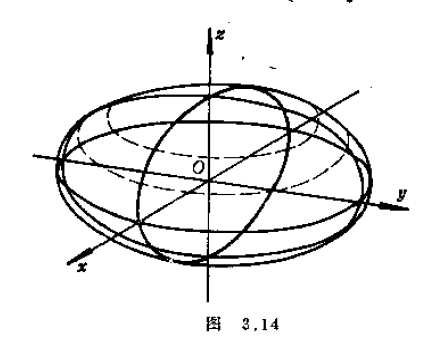
\includegraphics[width=0.42\linewidth]{ga-1010/ga-4.png}
\end{center}

\end{document}

\end{document}
